\documentclass[]{article}

\usepackage{graphicx}
\usepackage{float}
\usepackage[a4paper,top=2.5cm,bottom=2.5cm,left=2.5cm,right=2cm]{geometry}
\usepackage{subcaption}
\usepackage[table,xcdraw]{xcolor}
\usepackage{makecell}
\usepackage{tabularx}
\usepackage{enumitem}

\setlength{\tabcolsep}{13pt}
\renewcommand{\arraystretch}{2.3}


\begin{document}
	\pagenumbering{gobble}
	
	\begin{figure}[H]
		\centering
		
\includegraphics[scale=0.29]{FrontPage.png}
	\end{figure}
	

	\newpage
	\pagenumbering{arabic}	


	\tableofcontents
	
	\newpage
	
	
	\section{Introduction}
	
	\subsection{Purpose}
	The purpose of this document is defining the main design principles of the CLup software system, taking as input the concepts defined in the RASD. This document treats many topics regarding the software design. It starts from the high-level architecture choices and continues with the description of the main components, also describing how they interact with each other. The last section is about the system implementation, integration and the testing phases, useful to the developer to put together the various design aspects during the system development. 
	\\The reader can find a more detailed list of the treated topics in section 1.3.6.
	
	
	\subsection{Scope}
	
	\begin{paragraph}
		\newline
		CLup is an application that aims to provide the users with the possibility to queue to enter in a store, preserving as much as possible their safety and health. The lining up procedure can be done in two different ways: nearby the store with a physical ticket or from the application, where a virtual ticket is generated. In this way the crowd in the neighborhood of the stores is reduced, and so as a consequence the risks to get in touch with other people is decreased too. People lining up from home will start approach the store only when the system provides them a notification. Customers will then enter the store only when their turn has come, by the recognition of the QRcode on their ticket.\\
		This application is built in order to be as easy as possible so that it can be used by customers of all the ages. Customers can simply line-up to the store they prefer, but they can also take advance of other services that are implemented inside the book a visit feature. Store managers have a different interface to deal with the system, as they have different things to check and for sure different goals, such as monitor entrances/exits and then allow more people in the store if it is possible. \\
		However, more specific and deep descriptions of the available features can be found in the RASD document.\\
		
	\end{paragraph}

	\subsection{Definitions, Acronyms, Abbreviations}
	
		In this section we explain the meaning of some technical terms used in the document.
		
		
		\subsubsection{Definitions}
		
			\medskip
			
			\begin{tabular}{|c|l|}
				\hline
				\rowcolor[HTML]{DCDCDC} 
				\textbf{QR CODE} & \makecell[l]{A \textit{Quick Response code} is a kind of bar-code, readable by machines to retrieve \\information} \\ \hline
				\textbf{prova} & \makecell[l]{prova} \\ \hline
				\rowcolor[HTML]{DCDCDC} 
				\textbf{prova2} & \makecell[l]{prova} \\ \hline
			\end{tabular}
		
		
		\subsubsection{Acronyms}
		
			\medskip
			
			\begin{tabular}{|c|l|}
				\hline
				\rowcolor[HTML]{DCDCDC} 
				\textbf{RASD} & \makecell[l]{A \textit{Quick Response code} is a kind of bar-code, readable by machines to retrieve information} \\ \hline
				\textbf{DD} & \makecell[l]{Design Document} \\ \hline
				\rowcolor[HTML]{DCDCDC} 
				\textbf{GPS}& \makecell[l]{Global Positioning System} \\ \hline
			\end{tabular}
		
		
		\subsubsection{Abbreviations}
						
			
		\subsubsection{Revision History}
		
		
		\subsubsection{Reference Documents}
		
		
		\subsubsection{Document Structure}
		
			Here a list of the topics treated in each chapter of this Design Document.
			
			\paragraph{Chapter 1} is an introductory chapter, where are presented the purpose and the scope of this document. It also includes tables about acronyms and technical definitions.	
			
			\paragraph{Chapter 2} is the core of the Design Document. Here we can find the main architectural decisions, starting from the high-level design patterns. Then, there's a description of every single components and the interaction with each other. Lots of diagrams are included among the different subsections to better explain the presented concepts.
			
			\paragraph{Chapter 3} presents a deep description of the User Interface by means of a large number of detailed mockups and UX diagrams.
			
			\paragraph{Chapter 4} contains the strongest link to the RASD. In fact, it shows a mapping between the requirements presented in the RASD and the architectural components presented in chapter 2.
			
			\paragraph{Chapters 5} aims to give to the developers the guidelines of the implementation, integration and test phases, from both an high-level and a low-level point of view.
		
			\paragraph{Chapters 6 and 7} contains respectively tables about the effort spent by each group member in writing this document and the document references.
			\newpage
			
		
		\section{Architectural Design}
			
			\subsection{Overview}
				\begin{paragraph}
					\newline
					Three logic layers define the architecture of the application. This division has been made so that eventual needed updates that are related to only one of the parts does not affect the other two, leaving them independent from this point of view. The application has to be made in the Client-Server behavior, where the clients can join from different devices and work on the system through some hardware and software components that will be better explained into details in the next sections of the document. The three discussed layers are:\\
					\begin{itemize}
						\item Presentation Level (P) : it’s the higher level of the application and deals directly with the users. It shows to the users the actions they can do in a specific moment and so it has to display them the info in a well-ordered and understandable way. All the features and functions need to be made properly available when needed\\
						\item Business Logic or Application Layer (A) :  it’s the intermediate level the application and so it handles the data between the other two layers, checking and elaborating them so that the logic and the functionalities of the application are preserved and handled in the right way.\\
						\item Data Access Layer (D) : It’s the level that assures to keep data independent to the logic of the application. It handles the info with respect to the databases of the system, managing them when requested by the layer on its top.\\ \newline
					\end{itemize}
					
					
					Ideally, the sequence of the process begins with the request of the user to do a specific action when he wants to apply for a displayed available functionality, and to do this he will set the activation of a specific method that will trigger the application logic to manage it.
When the user concludes his procedure to being inserted in the queue of a store, sends a request to the server that handles the received data: if the lining-up has been made from home then the virtual ticket (its data) will be sent to the user, otherwise If the request of the ticket has been made from the totem at the store, the data sent back from the server will contain a valid or not valid ticket (the logic takes care of how many physical tickets have already been released and stops  sending valid tickets if the threshold has been reached yet).\\
					\newline
What’s more, for what concerns the users, every time they select and submit their preferences (mean of transport, favorite products, …) they will send data to the server, which makes them stored in the databases and allows the user to proceed through the next steps of the lining up procedure. Stored data will be useful when the user requests to see his statistics: they will be elaborated and sent back to the user, that would see them displayed on the screen of his device.\\
					\newline
The system has to deal with store managers too, and so the server will periodically update the available data of the manager, that would monitor the situation of the store in real time: this will allow the manager to send the request to allow more people enter the store, handled by the application logic and whose results are displayed back to the manager. \newline

\large //TODO HIGH LEVEL DIAGRAM with EXPLANATION
\newpage
				
				\end {paragraph}
				
<<<<<<< HEAD
	\subsection{Component view}
	\textbf{} \newline
	\textbf{Component Diagram} \newline
	In the current section will be explained the interactions of the various components that the system contains. The component view diagram allows to better understand the flow in the \textbf{Application Server}, which is organized in multiple subsystems so that the different competence areas are properly divided with respect to the functionality they’re built for.\\
The various components can communicate with each other through different interfaces. 
There are three components in the client side are the \textbf{customer} and the \textbf{store manager apps} and the \textbf{totem} where people take their physical ticket, which is connected to the application server too. The \textbf{Router} takes care to redirect to the proper subsystem or component the requests and responses that are generated during the lifetime of the system.\\
In the Application Server the \textbf{StoreHandler} and the \textbf{CustomerHandler} components are made so that they can handle the basic functions of the communication between the system and the store on one hand and between the system and the customer on the other one. General apps notifications and features that are not included in the ones that populates the queuing and book a visit subsystems rely here. In this way, if the system will handle and implement in the future some other small possible functions, these two components could be the ones that could handle the communications to guarantee to the store managers and the customers the best experience possible in the application.\newline\newline
What’s more, the application server is connected to:\\
	\begin{itemize}
		\item 	\textbf{QRcodeManager}: it cares about the generation of the tickets.
		
		\item 	\textbf{StoreSlidingDoors}: it allows to open the doors of the shop if the scanned ticket is valid.
		
		\item 	\textbf{GoogleMapsService}: it is necessary to retrieve data about the position of the store and of the customer.	
	
	\end{itemize}
	
	\textbf{} \newline
For the sake of completeness it has been shown also the \textbf{DBMS service}, but the main focus is made towards the Application Server, which is the core of the application’s logic. \newline\newline
In the following paragraphs the various subsystems will be briefly explained.\\

	\begin{figure}[H]
			\centering
			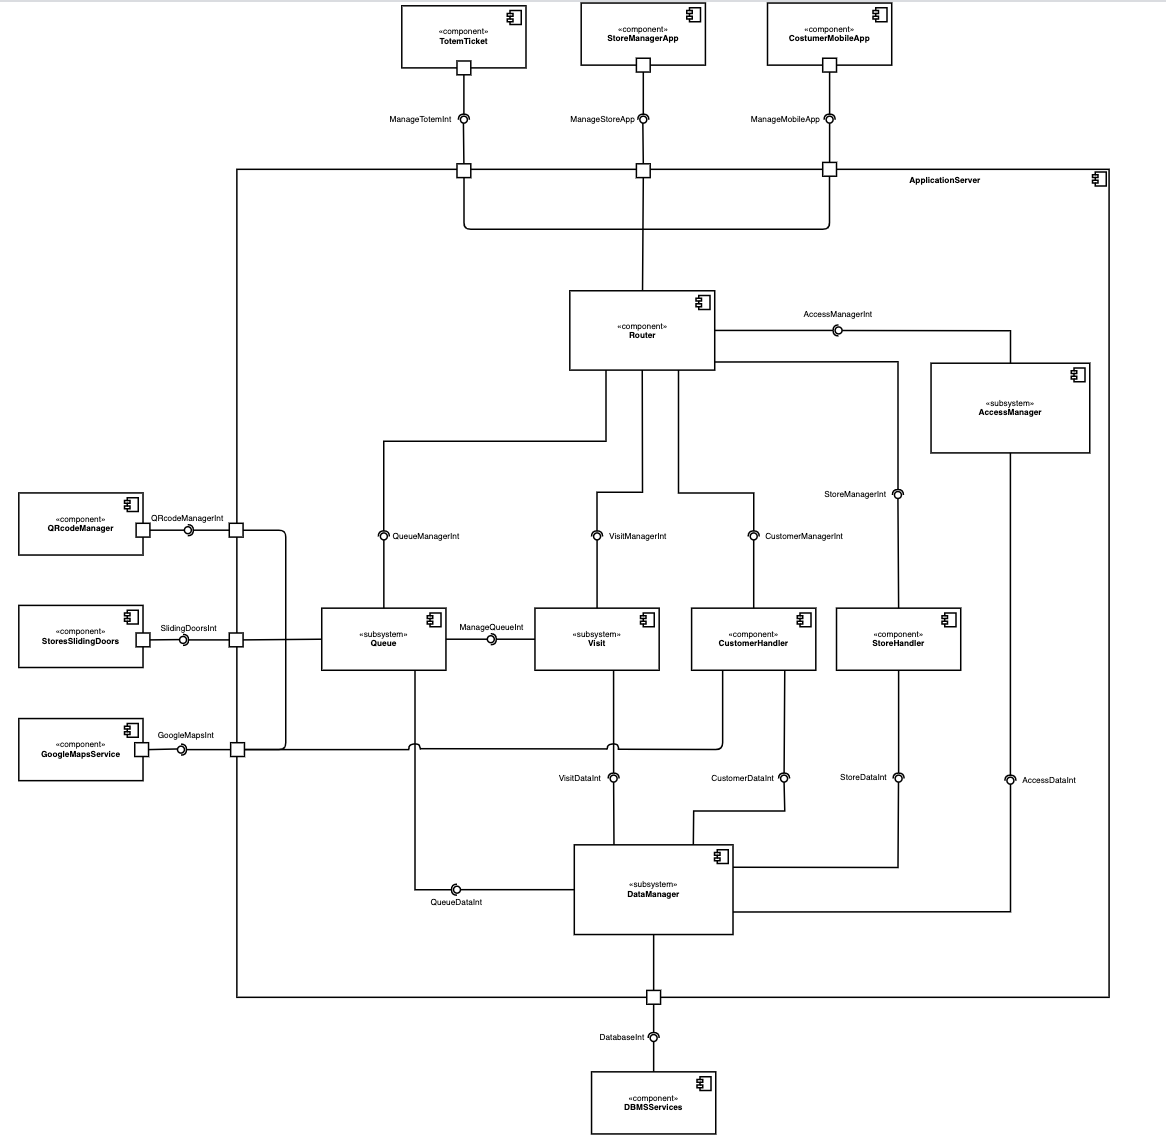
\includegraphics[scale=0.6]{ComponentView/ComponentViewDiagram.png}
			\caption{General Component Diagram}
			\label{fig:ComponentDiagram}
		\end{figure}
		\bigskip\bigskip


	\textbf{Access Manager subsystem} \newline
	The access manager cares about the sign up and the login of the users, both the customers and the store managers. The access is handled differently for the two entities, that have to provide different kind of information (the signing up and the authentication is different if the user is a store, because the system needs to accurately verify through some given documents the validity and the existence of the shop, while the sign up of a customer is more immediate because an existent valid email and a password would be sufficient), and the access to the data manager can be made with different purposes: with the sign up data are stored in the database, so that users are registered to the system, while with the login the validity of the inserted data (username and password) are checked with the ones that are already stored in the DB. 

	\begin{figure}[H]
			\centering
			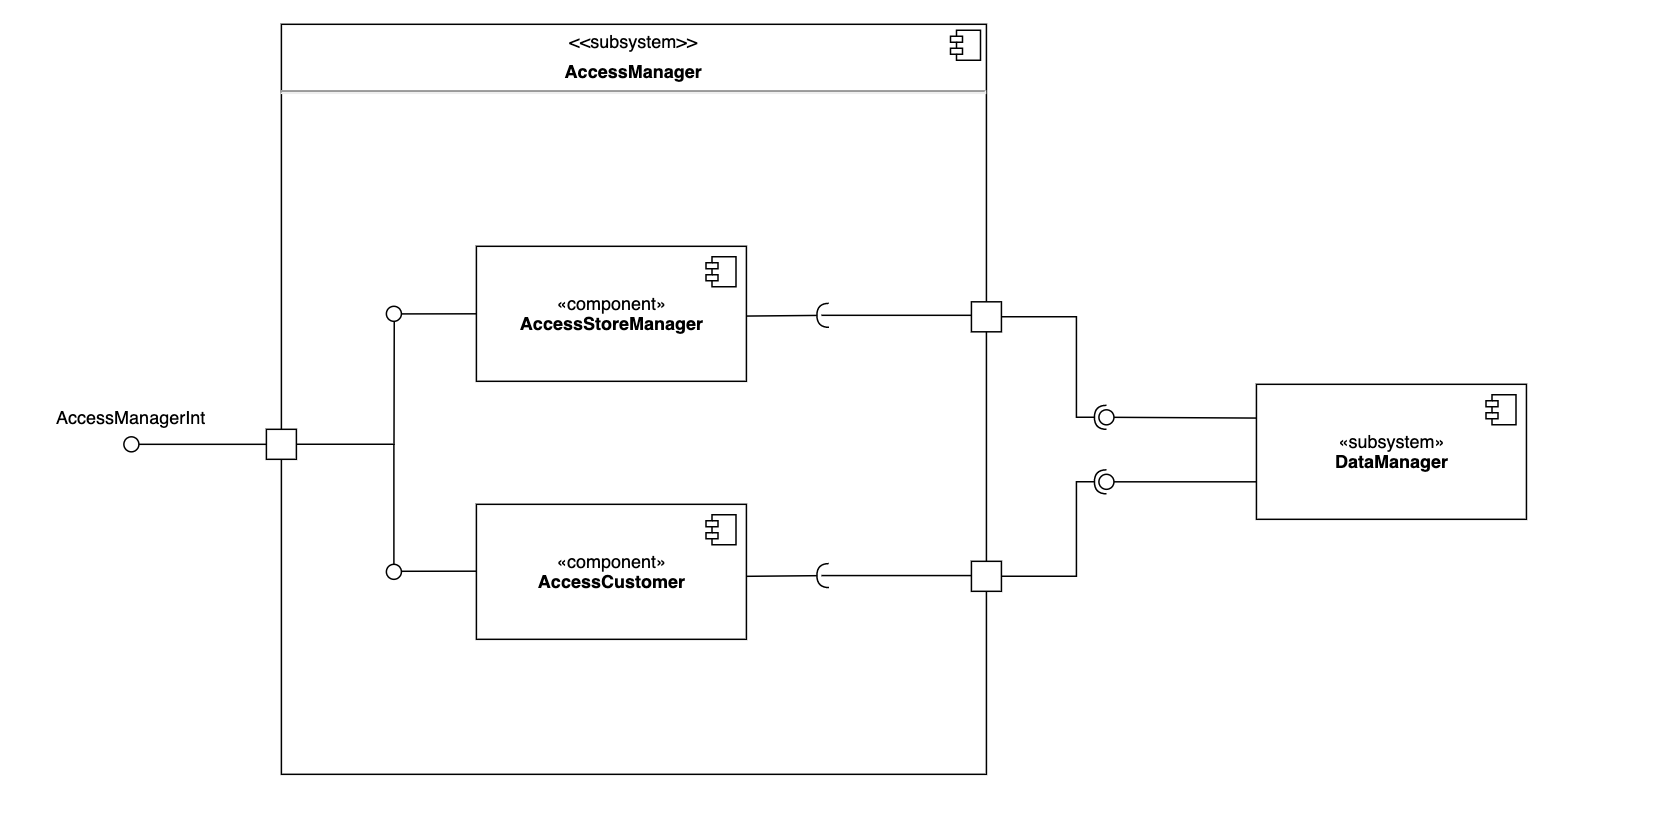
\includegraphics[scale=0.6]{ComponentView/AccessManagerComponent.png}
			\caption{AccessManager subsystem component diagram}
			\label{fig:AccessManagerDiagram}
		\end{figure}
		\bigskip\bigskip
	
	
	\textbf{Queue subsystem} \newline
	The Queue subsystem is the part of the system devoted to handling the people queueing to the store.
	Its responsabilities concern updating and managing the queue of people to a certain store, provide notification to users when they need to start approaching the store and handle the creation/recognition of Qr code tickets interfacing with an external module.
	The Queue subsystem is composed of three main components:
	
	\begin{itemize}
		\item 	\textbf{QueueHandler} is devoted to handling the queue logic beside of the application. It is responsible for putting users in the queue as well as removing them when their turn has come. It interacts with the Data Manager to store data about the queue and with the Sliding door interface to lock/unlock the door accordingly to Qr code scannings.
		
		\item 	\textbf{NotificationService} takes care of notifing CLup users when they need to reach the store. It interfaces with GoogleMapsAPI in order to estimate the time a user needs to reach the store given his position and transport mean.
		
		\item 	\textbf{Ticket Manager} is responsible for interfacing with the external software component \textit{QrcodeManager} in order to create, assign and recognize Qr codes.
		
	
	\end{itemize}

	
	\begin{figure}[H]
			\centering
			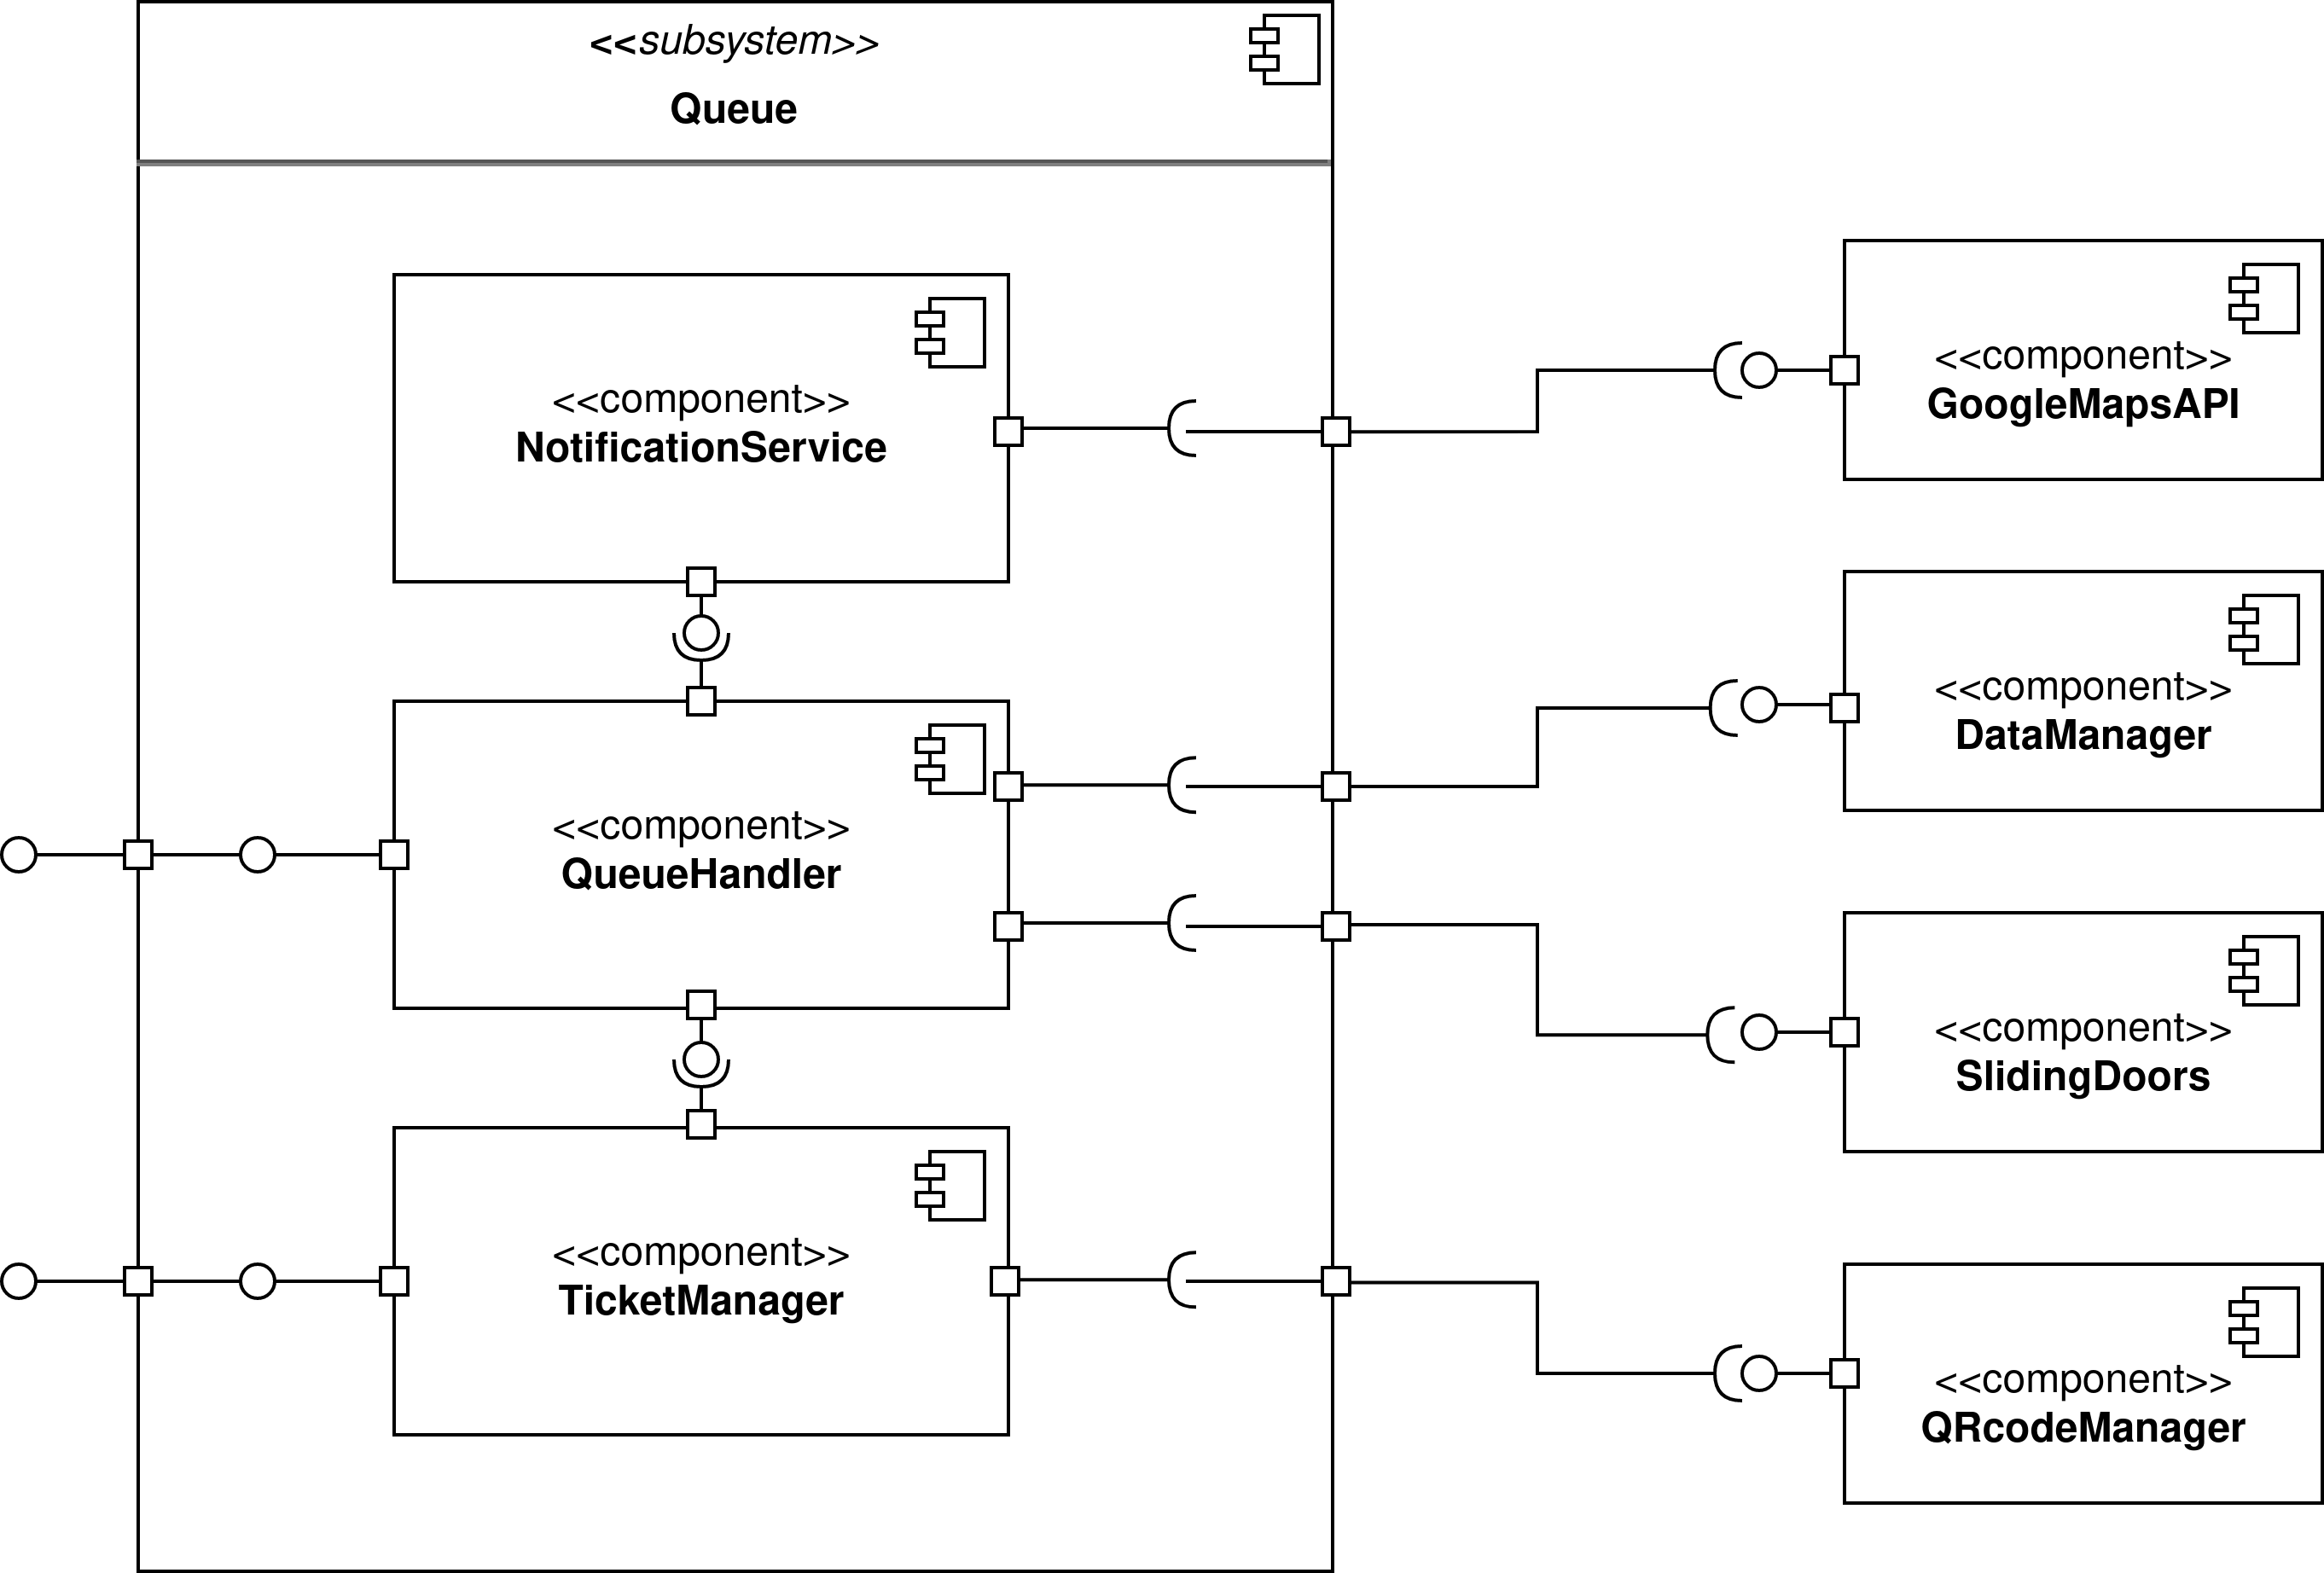
\includegraphics[scale=0.9]{ComponentView/queueComponent.png}
			\caption{Queue subsystem component diagram}
			\label{fig:Queuediagram}
		\end{figure}
		\bigskip\bigskip
		
			\textbf{} \\
	\textbf{Visit subsystem}
	\medskip \newline
	The visit subsystem aims to handle everything that is related to booking visits. It is composed by 4 components as the reader can see in the picture below. 
	
		\begin{itemize}
		\item \textbf{VisitHandler} works as an "orchestrator". It handles the requests that comes from outside the subsystem and exploits the functionalities offered by the other components;
		\item \textbf{StatisticHandler} collects user statistics;
		\item \textbf{SuggestionsHandler} computes suggestions based on user preferences and timetable availability;
		\item \textbf{TimetableHandler} handles time-slots and computes their availability.
	\end{itemize}
	

	\begin{figure}[H]
		\centering
		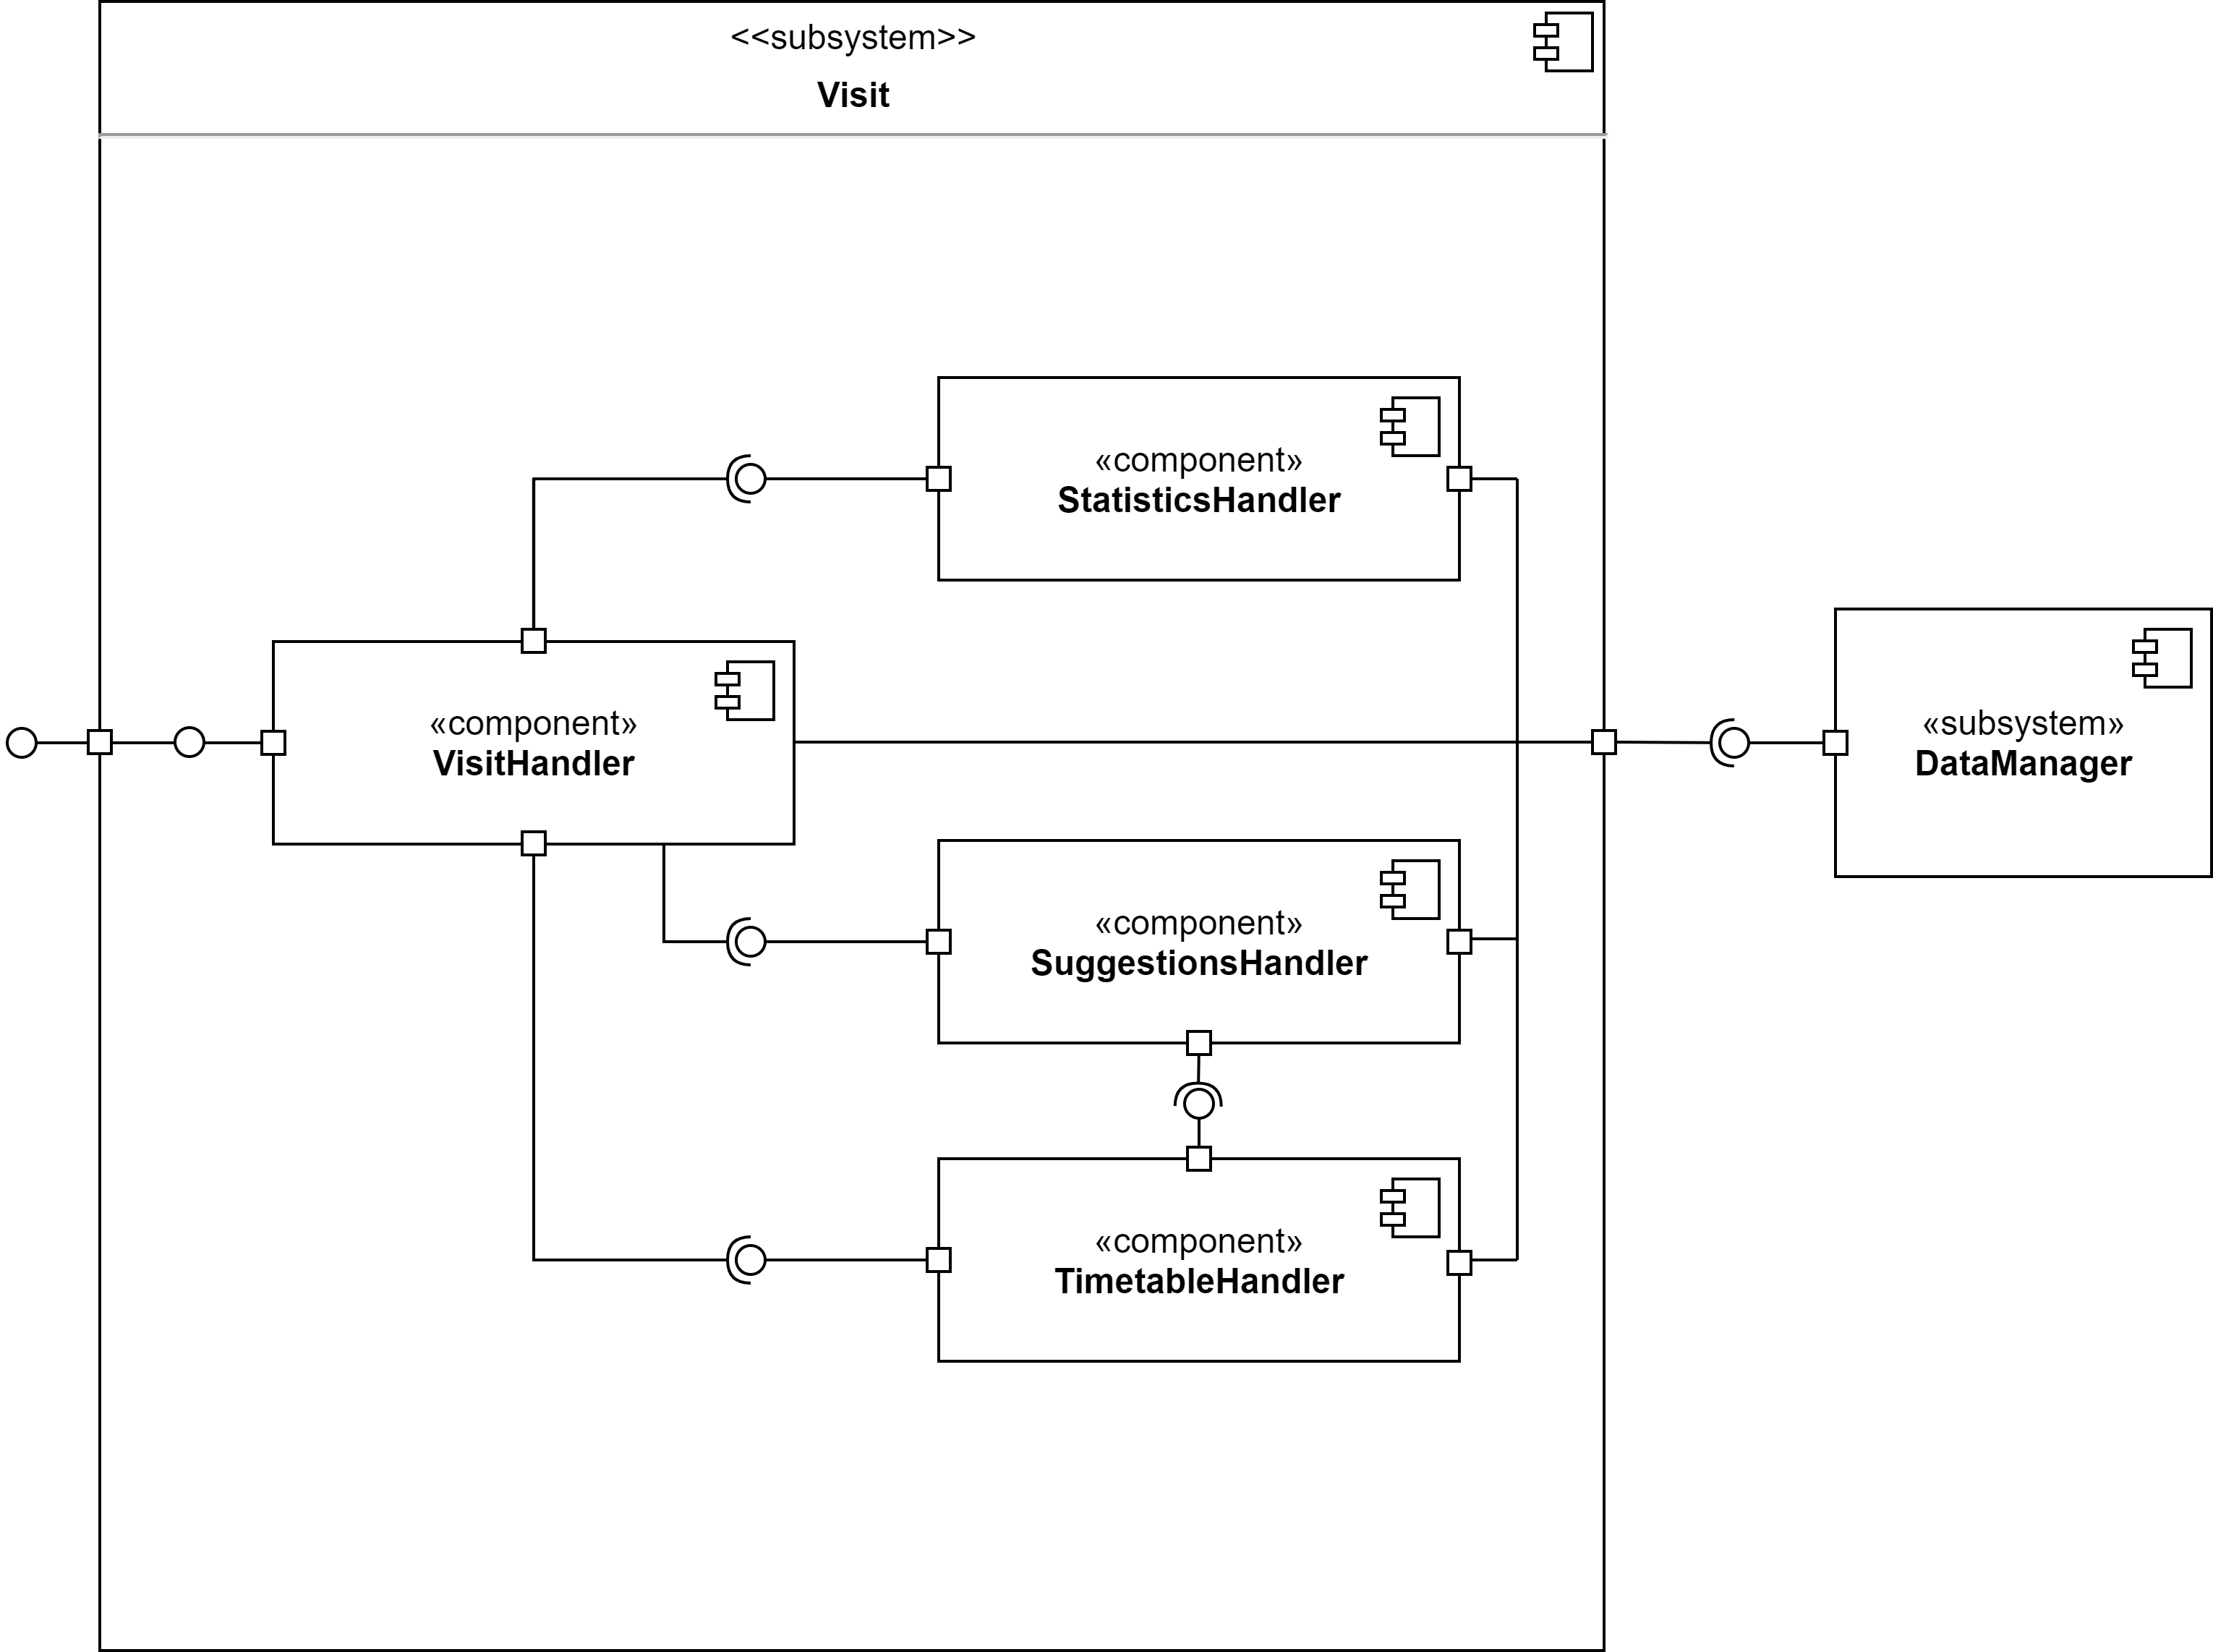
\includegraphics[scale=0.73]{ComponentView/VisitComponent}
		\caption{Visit subsystem}
		\label{fig:visitSubsystem}
	\end{figure}

		\bigskip\bigskip
		
		\textbf{Data Manager subsystem} \newline
		
		The purpose of the Data Manager subsystem is creating a common interface, shared with ther whole system, to access data stored in the database. \newline
		Instead of using directly the DBMS API, each component that needs to manipulate data that are stored in the DB is forced to use one of the two components that make the subsystem. \newline
		The reason behind this decision is to \textbf{decouple} our system from the DBMS: a change in the DBMS API or switching DBMS vendor will affect only our Data Manager subsystem instead of the whole application. \newline
		In particular:
		
		\begin{itemize}
		
			\item \textbf{DataRetriever} is devoted to data fetching
			\item \textbf{DataStorer} is responsible for storing data in the DB
		\end{itemize}
		
			\begin{figure}[H]
			\centering
			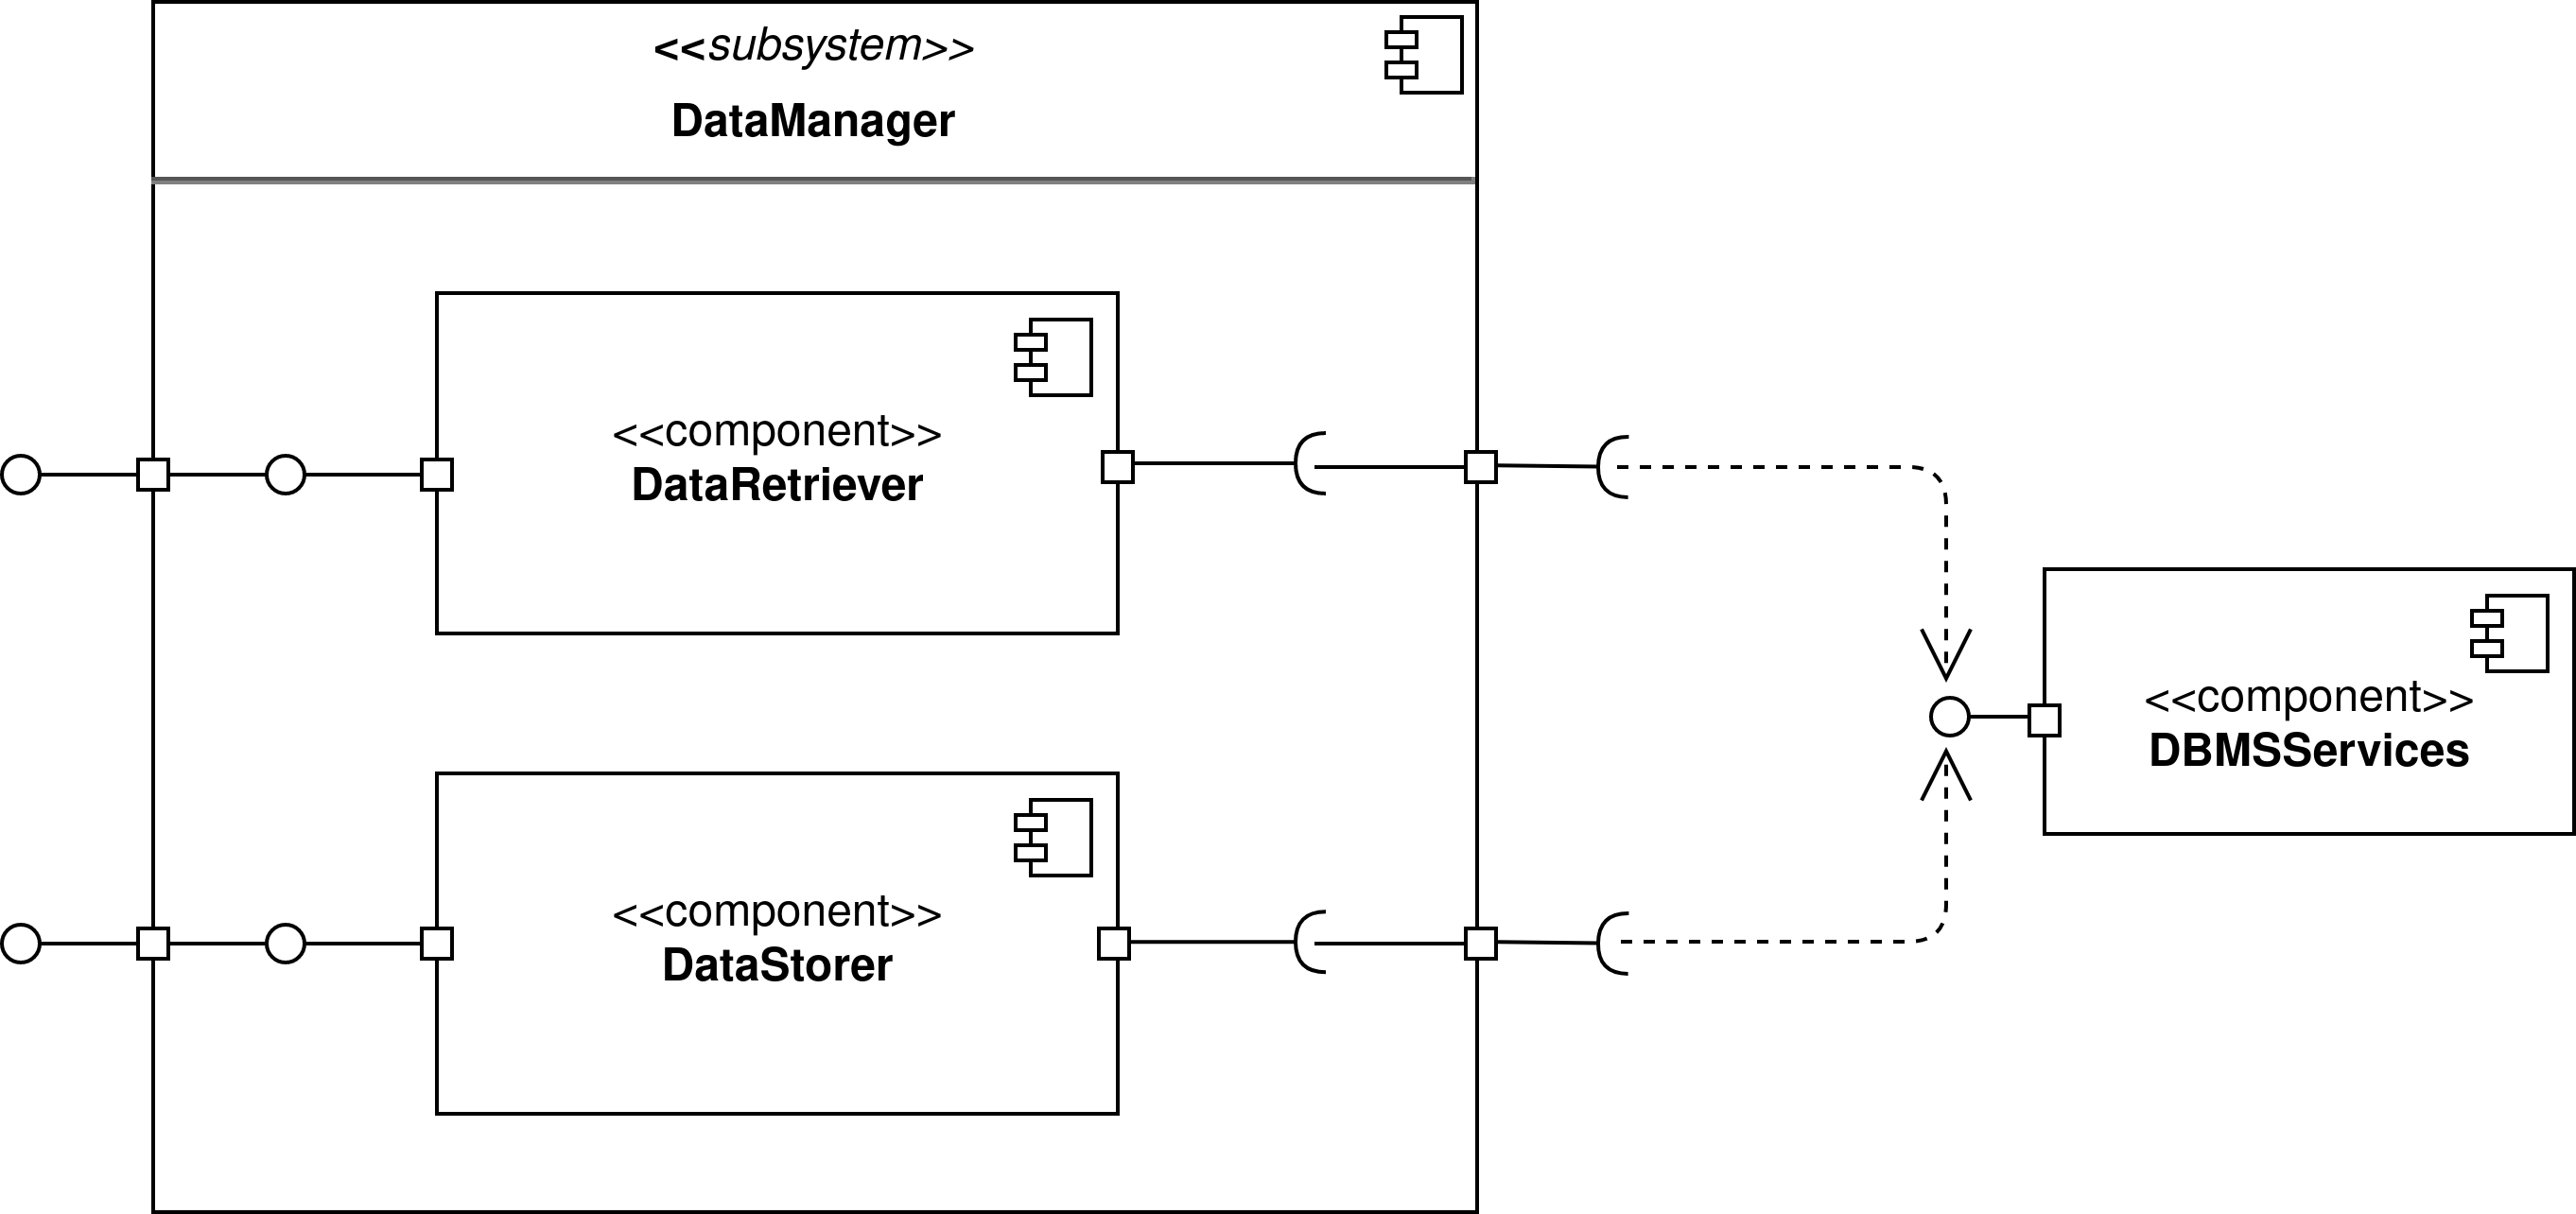
\includegraphics[scale=0.9]{ComponentView/DataManagerComponent.png}
			\caption{Data Manager subsystem component diagram}
			\label{fig:DataManagerDiagram}
		\end{figure}
	
		
	
	
	
	\subsection{Deployment view}
	\subsection{Runtime view}
	\subsection{Component interfaces}
	\subsection{Selected architectural styles and patterns}
	

				
	



	
				
	\newpage			
				
	\section{User Interface Design}
	This chapter aims to give a general idea of the user interface, both of the costumer mobile application and the store manager webapp. 
	This is done by means of mockups and UX diagrams.
		
		\subsection{Mockups}
		In the design process of the user interface the main guideline was the Requirement R2 (\textit{The user and manager applications are clear, intuitive and simple to use} - RASD). Therefore, the screen contains only the necessary components and the interaction with them is limited to a few of intuitive form and buttons.
		\\The presented mockups cover almost the totality of the screens you will find on the completed user interface. They show only the components needed to address the CLup goals, buttons such as "return to the previous screens" are not usually taken into account.
		
			\subsubsection{Mobile Application Mockups}
			\bigskip \bigskip \bigskip \bigskip
			\begin{figure}[h!] 
				\centering
				\subfloat[Sign-in screen]
				{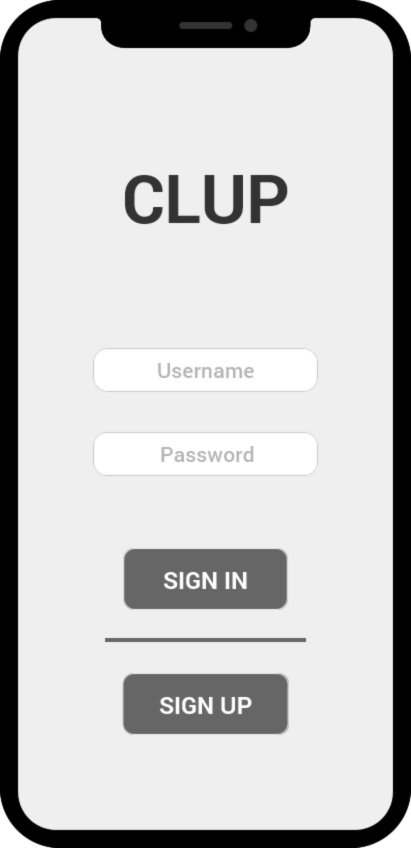
\includegraphics[width=.25\textwidth]{Mockups/signIn}}
				\qquad\qquad
				\subfloat[Sign-up screen]
				{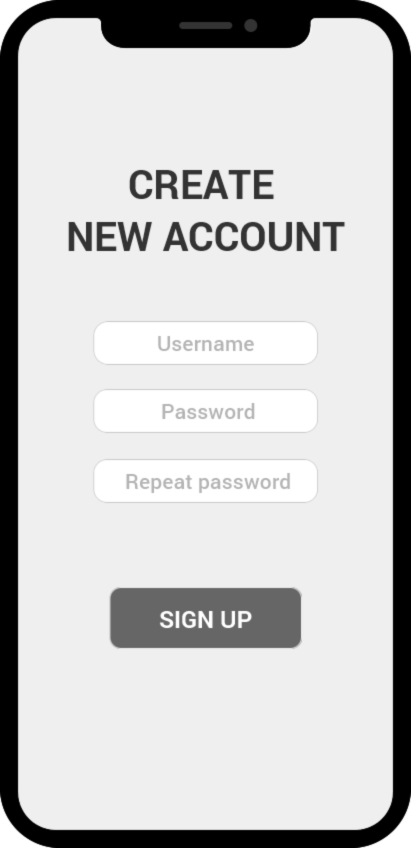
\includegraphics[width=.25\textwidth]{Mockups/signUp}}
				\qquad\qquad
				\subfloat[Store selection/booking check screen]
				{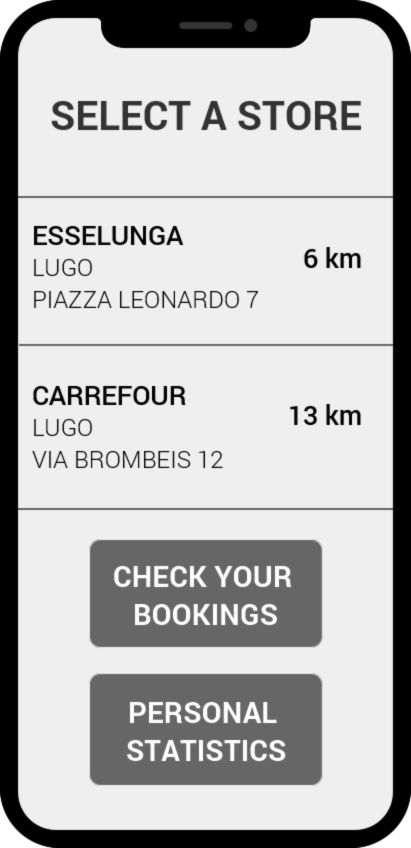
\includegraphics[width=.25\textwidth]{Mockups/selectStore}} 
			\end{figure}
		
			\newpage
			\begin{figure}[h!]\ContinuedFloat
				\centering
				\subfloat[Booking check screen]
				{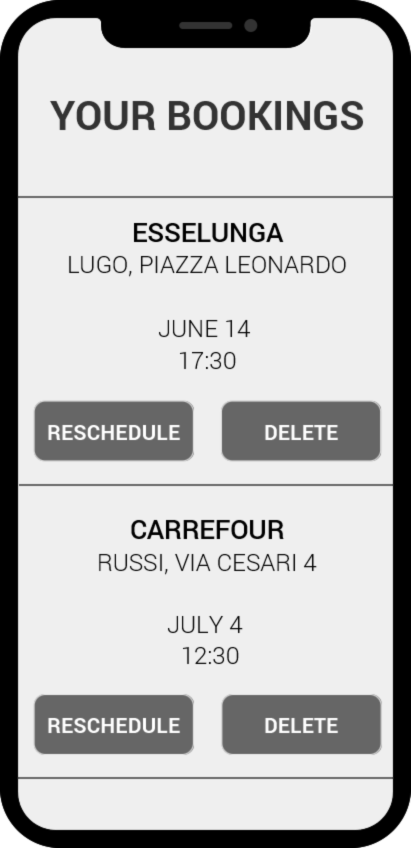
\includegraphics[width=.25\textwidth]{Mockups/bookingCheck}}
				\qquad\qquad
				\subfloat[Store available actions screen]
				{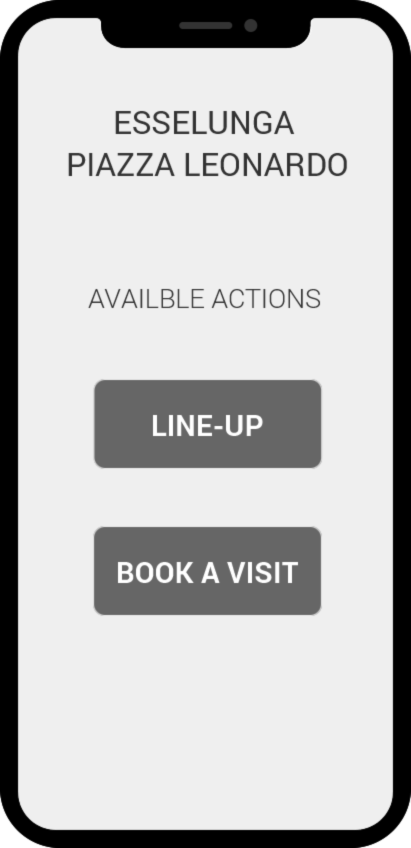
\includegraphics[width=.25\textwidth]{Mockups/storeAvailableActions}}
				\qquad\qquad
				\subfloat[Queue status screen]
				{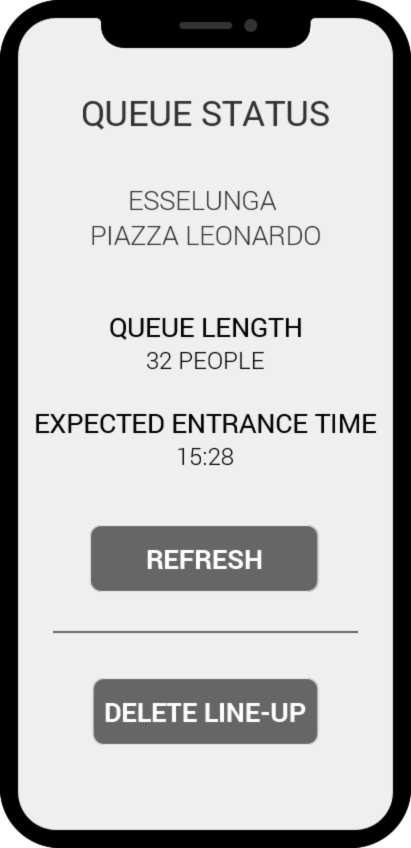
\includegraphics[width=.25\textwidth]{Mockups/queueStatus}} 
				
				\bigskip \bigskip \bigskip
				
				\subfloat[Book a visit screen]
				{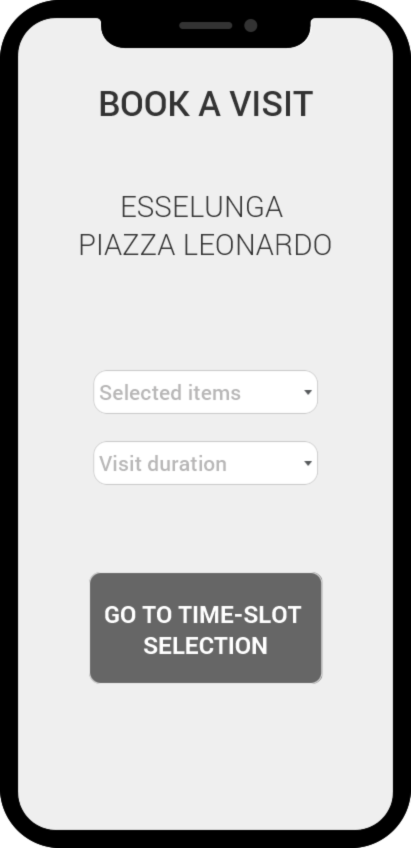
\includegraphics[width=.25\textwidth]{Mockups/bookVisit}}
				\qquad\qquad
				\subfloat[Time-slot selection screen]
				{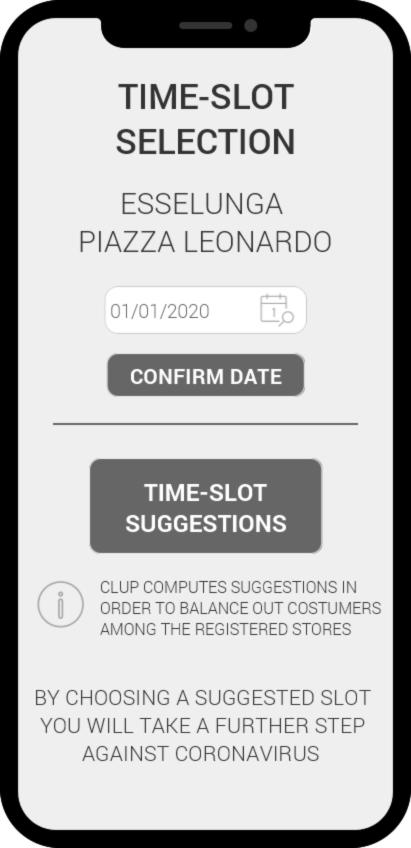
\includegraphics[width=.25\textwidth]{Mockups/timeSlotSelection}}
				\qquad\qquad
				\subfloat[CLup notification]
				{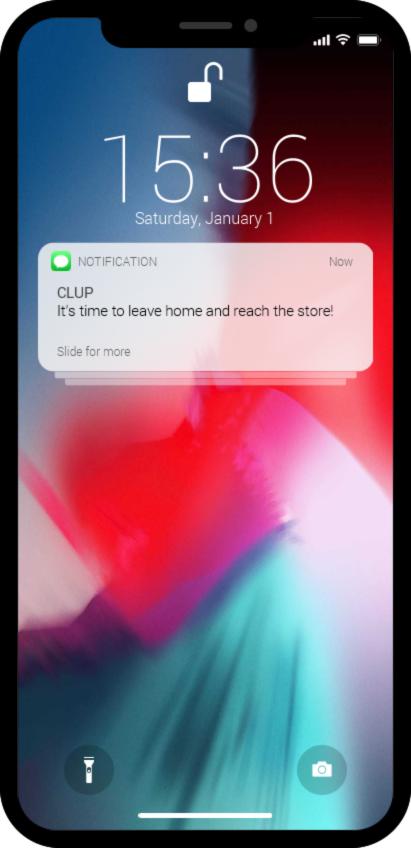
\includegraphics[width=.25\textwidth]{Mockups/notification}} 
			\end{figure}
		
			\newpage
			\subsubsection{WebApp Mockups}
			\bigskip
		
			\begin{figure}[H]
				\centering
				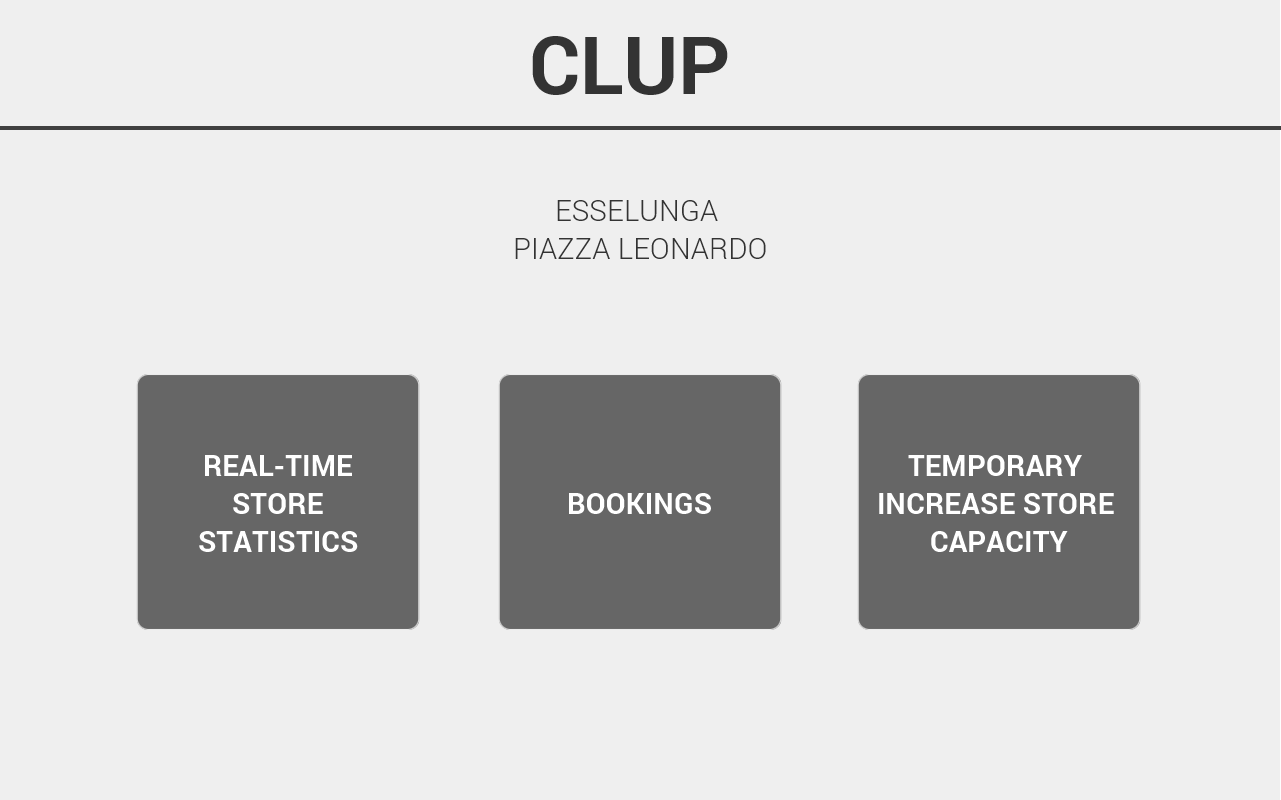
\includegraphics[scale=0.3]{Mockups/webAppHome}
				\caption{Home screen}
				\label{fig:homeScreen}
			\end{figure}
			\bigskip
			
			\begin{figure}[H]
				\centering
				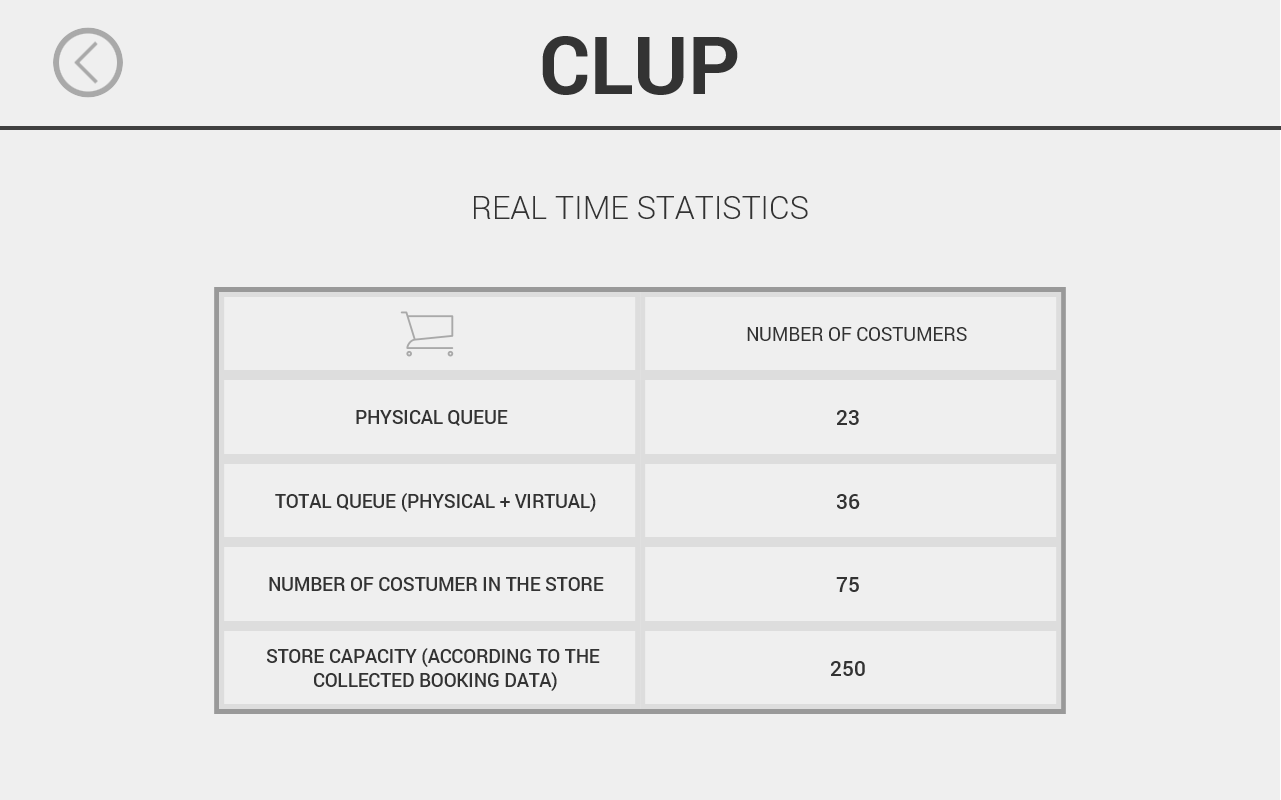
\includegraphics[scale=0.3]{Mockups/storeStatistics}
				\caption{Store statistics screen}
				\label{fig:Storestatisticsscreen}
			\end{figure}
		
			
			\begin{figure}[H]
				\centering
				\includegraphics[scale=0.3]{Mockups/storeBookings}
				\caption{Store bookings screen}
				\label{fig:ManagerHomeMockup}
			\end{figure}
		
		\newpage
		\subsection{UX diagrams}
		The chapter ends with two UX diagrams. They show the general flow of the screens giving more details on the user experience. "General" because some link between screens where omitted, like the "return" from a screen to the previous.
		
		\begin{figure}[H]
			
\includegraphics[scale=0.7]{UX diagrams/legend}
			\label{fig:MobileAppUXdiagram}
		\end{figure}
		\begin{figure}[H]
			\centering
			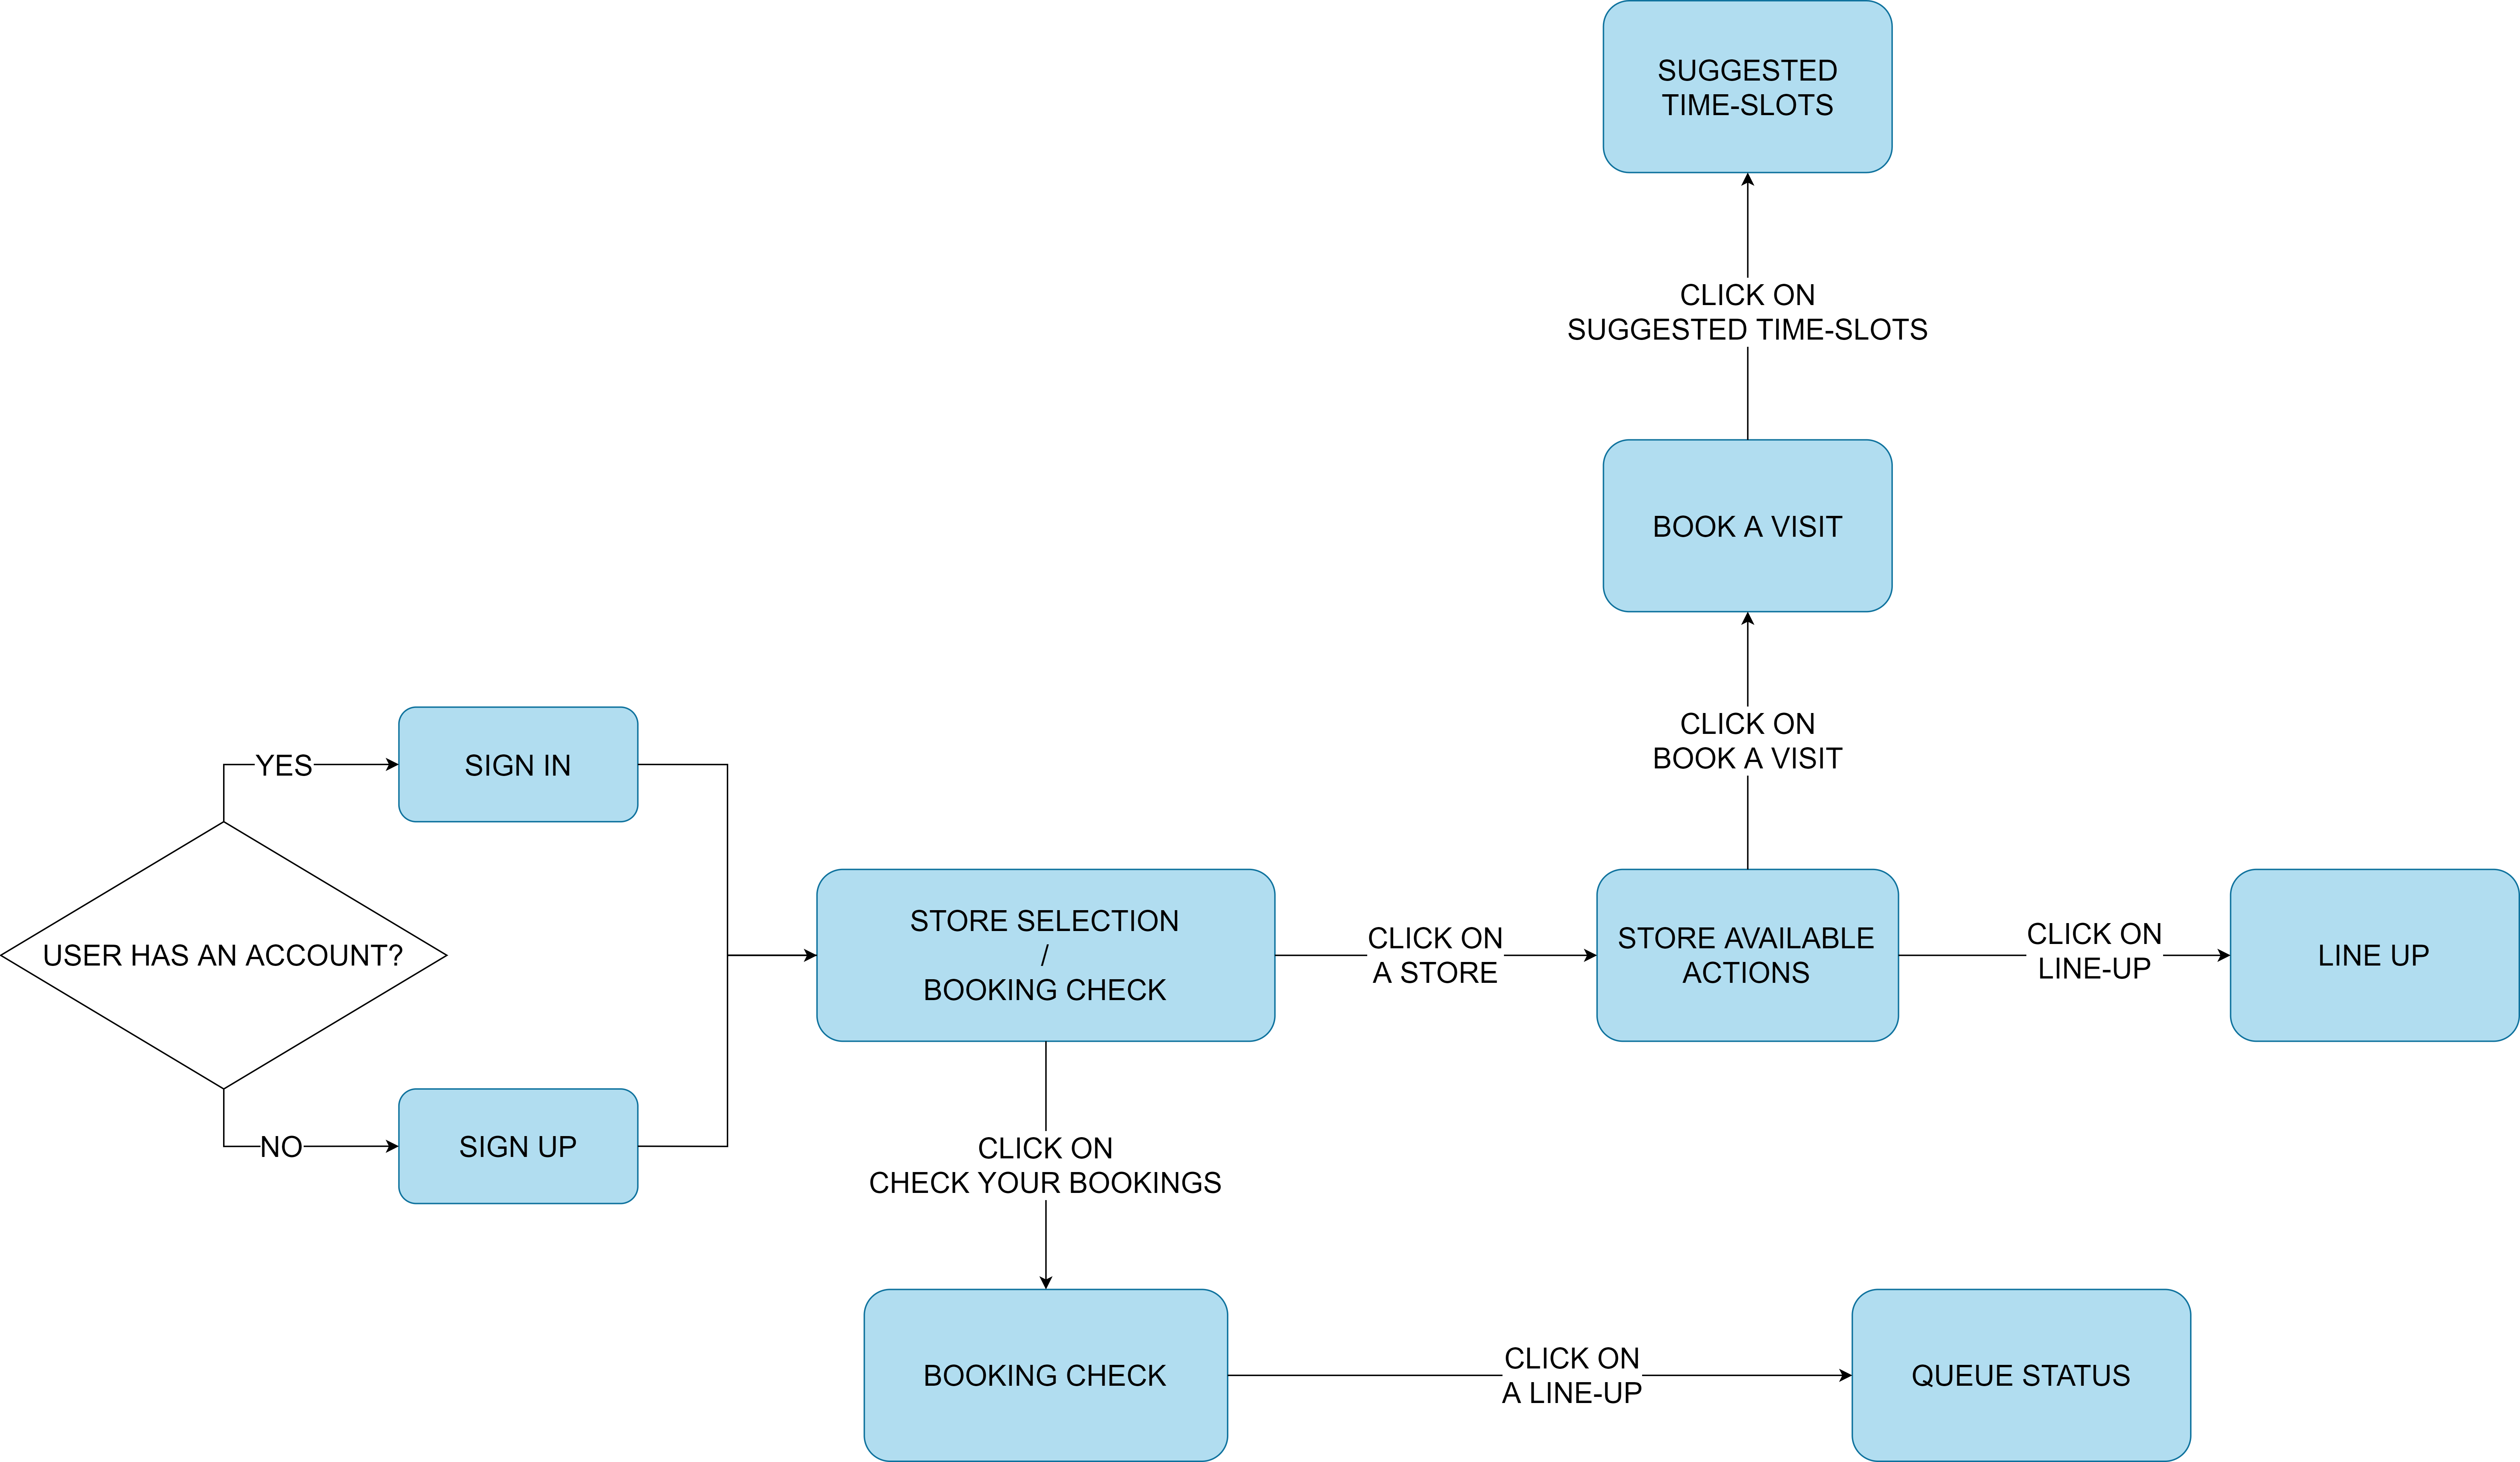
\includegraphics[scale=0.38]{UX diagrams/mobileApp}
			\caption{Mobile App UX diagram}
			\label{fig:MobileAppUXdiagram}
		\end{figure}
		\bigskip \bigskip \bigskip \bigskip
		\begin{figure}[H]
			\centering
			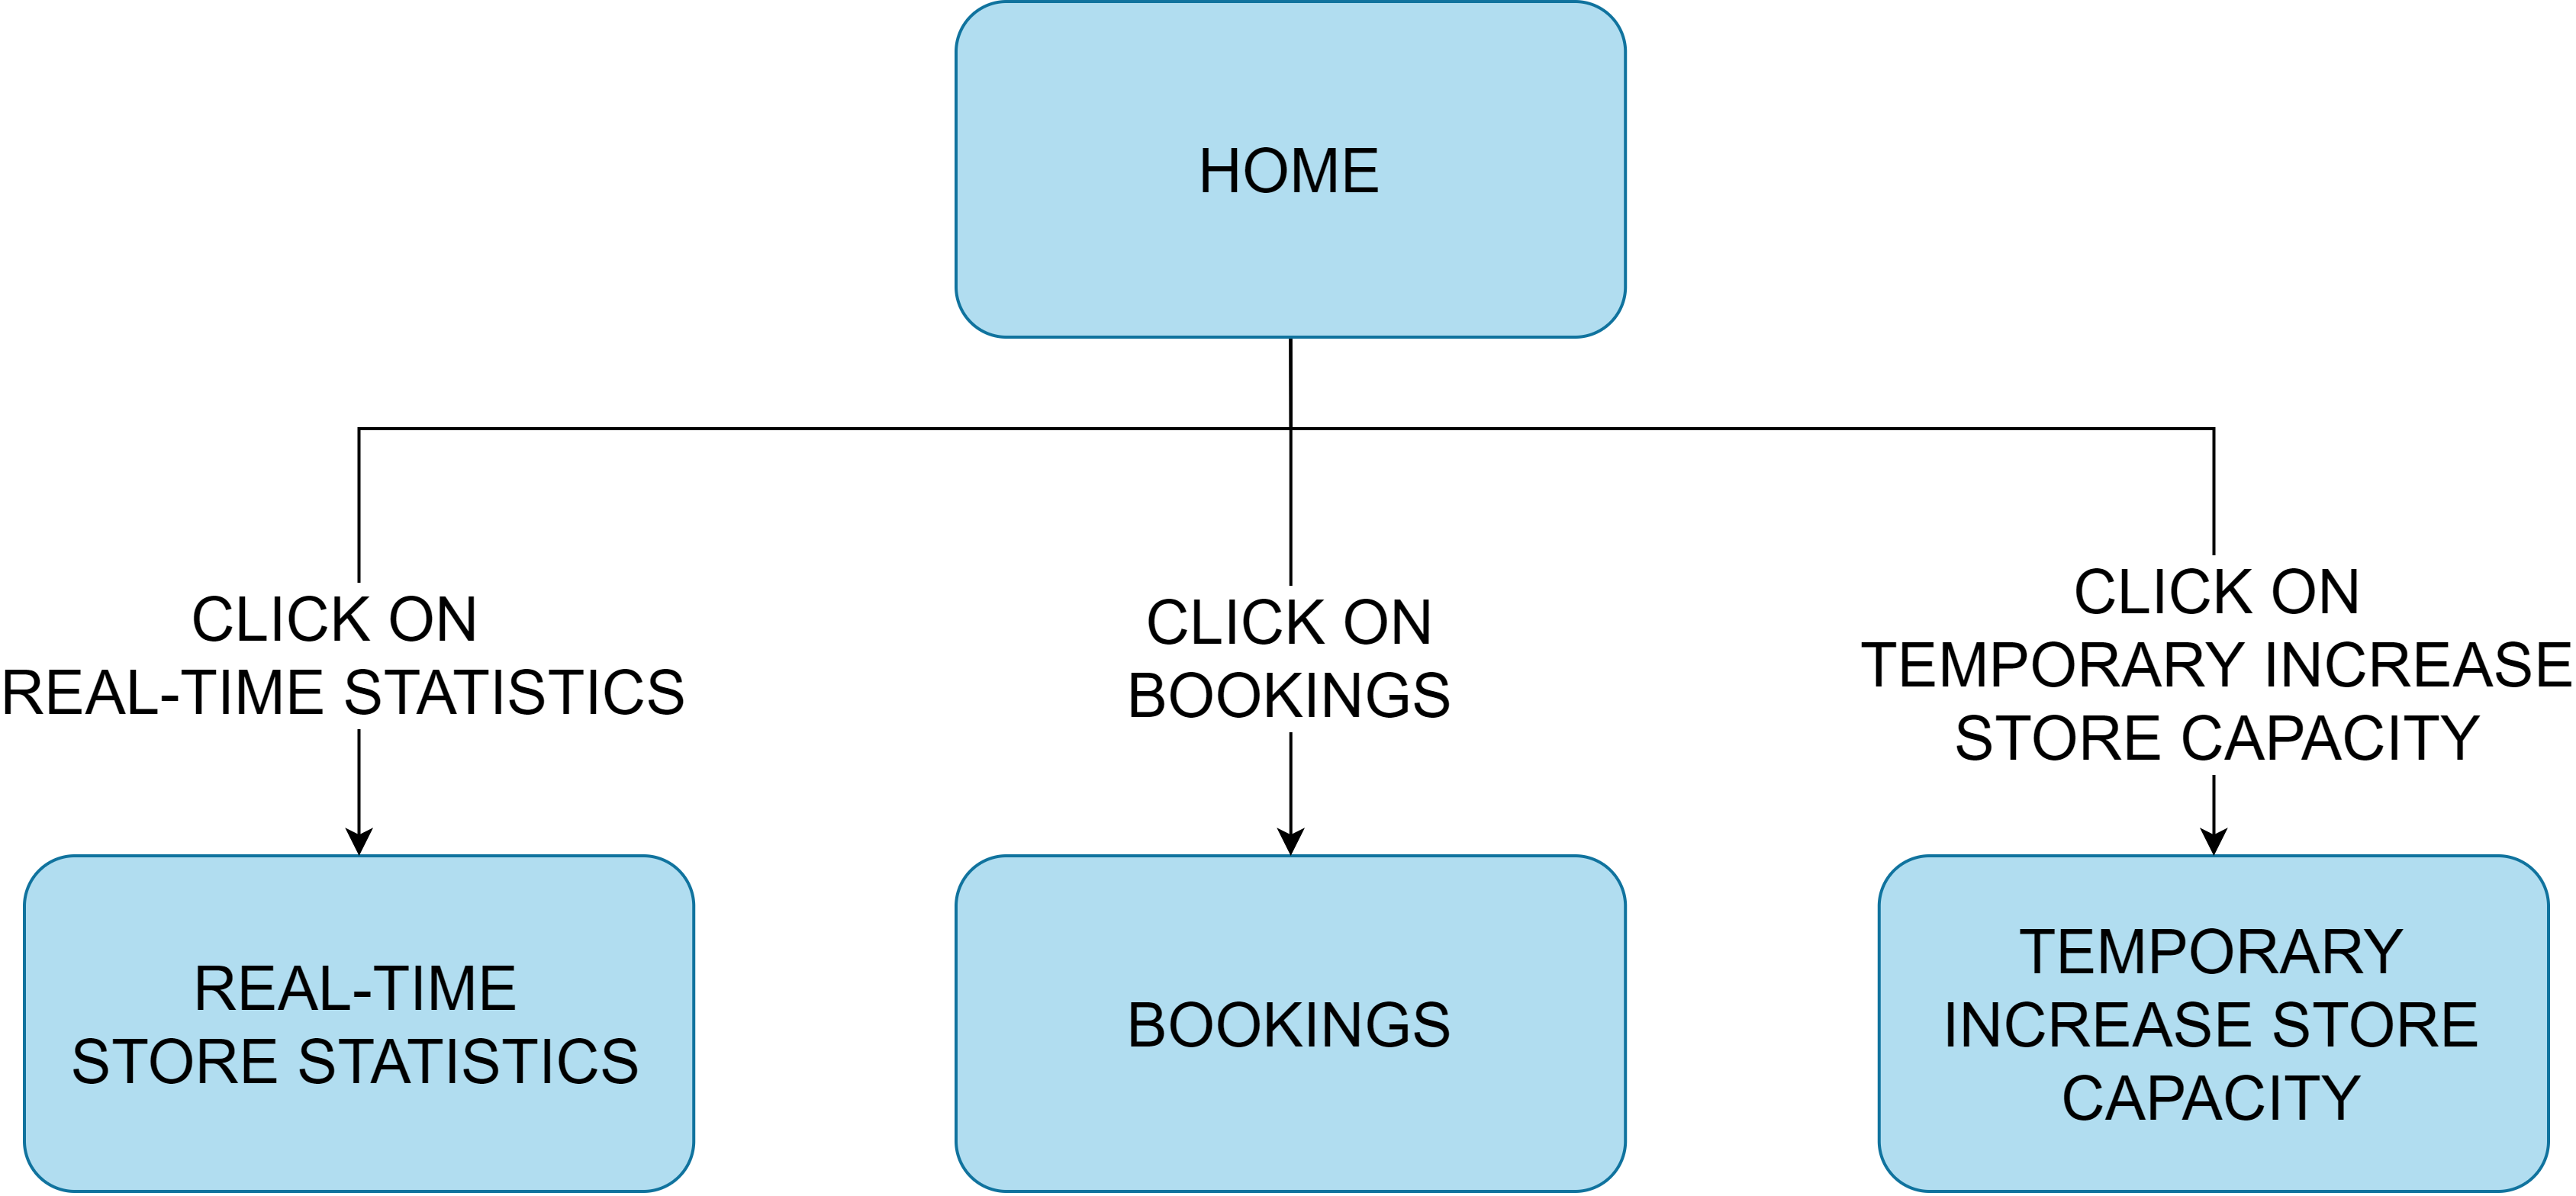
\includegraphics[scale=0.38]{UX diagrams/webAppHome}
			\caption{WebApp UX diagram}
			\label{fig:MobileAppUXdiagram}
		\end{figure}
			
		\newpage
		
		\section{Implementation, Integration and Test Plan}
			 \bigskip
			 
			 \subsection{Overview}
			 \medskip
			 Testing is an important practice to make sure that the system behaves as we expect and is able to fulfill the requirements and reach the goals that it is supposed to do. For this reason, the system should be divided in more than a unique block when it is implemented: testing the whole system only when its design has been finished is definitely not a good practice and will lead with every probability to high costs of repair. \\The various components of the system need to be checked independently and then gradually integrated one with the other, with other tests that are subsequent to their integration to make sure that the behavior is exactly what it is expected to be. Of course, it is impossible to find all the bugs in our system through testing, as we know that program testing can be used to show their presence, but not their absence. \\This is the reason why this part of verification and validation is very important: release an application that is as much bug-free as possible. It is important that the verification and validation phases start as soon as the development of the system begins in order to find errors as quickly as possible.\newline\newline
			
			\subsection{Implementation Plan}
			\medskip
			As a consequence of what has been said above and also taking into account that the CLup system is a relatively small one, then it needs to be implemented, tested and integrated following a bottom-up approach. As in unit testing, drivers must be constructed for each leaf module and then, as the system is built up, they will be replaced by higher level components that could use the lower level subsystems’ functionalities. Following this approach, it will be possible to parallelize implementation and the testing procedures.\newline

The external components can be assumed to be already reliable, as they are implemented and used without any specific improvements. So, this assumption can be valid for the GoogleMapsService, the StoreSlidingDoors and QRcodeManager components. The integration with the subsystems that interface with them has to be accurately tested and validated.\newline

The other components and subsystems that should be considered are the same ones that have been described and shown in the Component View section, that are listed below for the sake of reading them more confortably (the last three ones belong to the client side of the system):
				\begin{itemize}
					\item DBMS Services
					\item Data Manager subsystem
					\item Access Manager subsystem
					\item Store Handler
					\item Customer Handler
					\item Visit subsystem
					\item Queue subsystem
					\item Router
					\item CustomerMobileApp
					\item StoreManagerApp
					\item Ticket Totem
				\end{itemize}

The first components that have to be implemented and tested are the DBMSServices, because they are the ones that allow to keep system’s data updated to the last version and they allow to write on the Database, always recalling to make it persistent.\\ \newline
Then we can proceed with the Data Manager subsystem, that directly interfaces from the application server towards the DBMS Services and allows to ask and retrieve data through appropriate queries, or to send new data of new info collected during the users’ registrations or their submitted preferences.
Once the Data Manager has been completed, then the other subsystems can be built: Access Manager is independent from the other components, so it can be developed in parallel with other tasks. Because of its purpose, the only role that he has is to guarantee that accesses to the system are authenticated, and this function is perfectly isolated from the others.\\ \newline
In fact, when a customer wants to line up, he has only to face and interact with the Visit and Queue subsystems. Data that are necessary for the bookings and for queuing are retrieved from the Data Manager that takes them from the DB, and then inside the components are elaborated and proposed to the users. As already said, the two subsystems – Visit and Queue – do not interact with each other because as the more independent they are, the easier would be in the future to repair and modify them without having to handle other components as a cascade unwanted effect. \\ \newline
Then comes the turn of the Customer Handler and Store Handler components. As the functionalities to store data of a visit have been already implemented and they should properly work, now all the other type of queries of the customers and the store managers can be managed and processed (e.g. booked visits, real time statistics, temporarily increasing the store capacity, …), as their information can be already be stored in the DB.\\ \newline
The Router is the last component that is implemented and tested: its only role is to dispatch messages coming from different parts of the system and assures that they arrive to the right subsystem or component. It has only one main function, but it is very important for the correct behavior of the whole application.
From the point of view of the client components, they can be implemented in parallel to the application server and once the AS has been completely tested, then the two parts can be merged to see if the whole system complies with the requirements and the overall goals.\\ \newline
Finally, we can list what is the strict sequence of constraint of component implementation that must be fulfilled (the client side components and the Access Manager are not included in the following list because their implementation, as previously said, can be done in parallel with the others): 
				\begin{itemize}
					\item DBMS Service
					\item DataManager
					\item Queue subsystem
					\item Visit subsystem
					\item CustomerHandler and StoreHandler
					\item Router
				\end{itemize} 

			 
		\section{Effort spent}
			
			\medskip
			\textbf{\large Antonio Ercolani:} \\ \newline
			\begin{tabular}{|l|c|}
				\hline
				Purpose and Document Structure &  \textbf{1h} \\ \hline
				\rowcolor[HTML]{DCDCDC} 
				User Interface Design & \textbf{8h} \\ \hline
				
			\end{tabular}
			\newline
			\newline
			
			\medskip
			\textbf{\large Vittorio Fabris:} \\ \newline
			\begin{tabular}{|l|c|}
				\hline
				Scope and organization of chapter 1&  \textbf{1,5h} \\ \hline
				\rowcolor[HTML]{DCDCDC} 
				 Architectural Design Overview & \textbf{3h} \\ \hline
				 Component View & \textbf{7h} \\ \hline
				\rowcolor[HTML]{DCDCDC} 
				Validation and Testing & \textbf{5h} \\ \hline
			\end{tabular}
	
			
			\section{References}	
			
			
	

				
\end{document}
